\section{Effective One-Particle Theories}
\subsection{Hartree-Fock (HF)}

\newcommand{\hcore}{H^{\text{core}}_{\mu\nu}}
\newcommand{\ksveff}{V^{\text{eff}}_{\mu\nu}}

\subsubsection{The Hartree-Fock Equations}
The Hartree-Fock equations are a set of linear equations that couple spin orbitals in the determinant wavefunction. They can be obtained by minimizing the energy of a Slater determinant with the constraint that spin orbitals remain orthonormal. Using the method of Lagrangian multipliers, this constraint optimization problem can be converted to a set of linear equations, which take the form of an eigenvalue problem.
%, thus it is more concise to define the one-body operator on the left hand side as the Fock operator. (see eq.~(3.49) in Szabo).

To derive the Hartree-Fock equations, we use a Slater determinant to evaluate the total energy, then minimize it. Consider $N$ spinless fermions, labeled using $i,j,k,\dots$, in $N$ orbitals $\chi_a,\chi_b,\dots,\chi_N$. Given determinant wavefunction $\ket{\Psi_0}=\ket{\chi_a\chi_b\dots\chi_N}$ and electronic Hamiltonian made up of only one- and two-electron terms $\mathcal{H}=\sum\limits_{i=1}^N h(i) + \sum\limits_{i=1}^N\sum\limits_{j>i}^N v(i,j)$. The total energy is
\begin{align} \label{eq:sdet-energy}
E= \sum\limits_{a=1}^N [a|h|a] + \frac{1}{2}\sum\limits_{a,b=1}^N [aa|bb] - [ab|ba],
\end{align}
where $[a|h|a]$ denotes, and $[aa|bb]$ denotes~\cite{Szabo1996}.

Constraint minimization of eq.~(\ref{eq:sdet-energy}) with the extra requirement that each spin orbital is doubly occupied leads to the restricted Hartree-Fock (RHF) Fock operator. Its first $N/2$ eigenvectors are the spin orbitals in the lowest-energy Slater determinant. The lowest energy value can be obtained by a weighted sum of its eigenvalues according to the occupation of the spin orbitals.

\subsubsection{Minimum-basis H$_2$}

Instead of starting with the tedious derivation of the Fock operator and its iterative numerical solver, I will first show a concrete application of RHF to minimum-basis hydrogen molecule (H$_2$). %The minimum basis consists of two 1s functions, one centered at each nucleus $\{\phi_\mu\}$, $\mu=1,\dots,K$, where $K=2$.
On p. 140 of A. Szabo and N. S. Ostlund, the restricted Fock operator in any basis $\{\phi_\mu\}$ is written as
\begin{align}
F_{\mu\nu} = \hcore + \sum\limits_{a=1}^{N/2} 2(\mu\nu|aa) - (\mu a|a\nu),
\end{align} % (3.148)
where $a$ labels molecular orbitals, which are eigenstates of the Fock operator. We immediately note that the Fock operator is a peculiar one-electron operator that depends on its own eigenstates. A self-consistent solution to $F_{\mu\nu}$ typically involves guessing, checking and iterating.

$\hcore$ is the one-electron part of the Hamiltonian expressed in the given basis % (3.149)
\begin{align} \label{eq:hf-hcore}
\hcore = \int d\bs{r}_1 \phi_\mu^*(\bs{r}_1)\left(
-\frac{1}{2}\nabla_1^2-\sum\limits_A \dfrac{Z_A}{\vert\bs{r}_1-\bs{R}_A\vert}
\right)  \phi_\nu(\bs{r}_1).
\end{align}
The two-electron integral notation $(\mu\nu|\lambda\sigma)$ is defined by eq.~(3.155) in Szabo
\begin{align} \label{eq:hf-eri}
(\mu\nu|\lambda\sigma) = \iint d\bs{r}_1 d\bs{r}_2 \phi_\mu^*(\bs{r}_1)\phi_{\nu}(\bs{r}_1)
\frac{1}{\vert\bs{r}_1-\bs{r}_2\vert}
\phi_\lambda^*(\bs{r}_2)\phi_\sigma(\bs{r}_2).
\end{align}
The first term in the sum of eq.~(\ref{eq:roothaan-fock})
\begin{align}
J_{\mu\nu} \equiv (\mu\nu|aa)
\end{align}
is often called the Coulomb or direct operator, because it describes the Classical density-density interaction of charged particles having density distribution $\phi_a^*(\bs{r}_2)\phi_a(\bs{r}_2)$. The second term
\begin{align}
K_{\mu\nu} \equiv (\mu a|\nu a)
\end{align}
is the exchange operator and has no classical interaction. The exchange-correlation contribution to the Fock matrix is sometimes called the Hartree-Fock effective potential operator
\begin{align}
\ksveff\equiv 2J_{\mu\nu} - K_{\mu\nu}.
\end{align}

Suppose each molecular orbital $a$ is written as a linear combination of the basis functions
\begin{align}
\psi_a = \sum\limits_{\mu=1}^K C_{\mu a} \phi_\mu,
\end{align}
then the Fock operator can be written as (from Roothaan equations)
\begin{align} \label{eq:roothaan-fock}
F_{\mu\nu} = \hcore + \sum\limits_{\lambda\sigma} P_{\lambda\sigma} \left[
(\mu\nu|\sigma\lambda) - \frac{1}{2}(\mu\lambda|\sigma\nu)
\right],
\end{align} % (3.154)
where $P_{\lambda\sigma}=2\sum_{a=1}^{N/2} C_{\lambda a}C_{\sigma a}^*$ is the density matrix. % (3.145)

Conceptually, the simplest approach would be to use the ground-state wavefunctions of the two hydrogen atoms as the basis for the hydrogen molecule. We can guess the ground-state wavefunction of the hydrogen molecule. First, the spins of the two electrons anti-align, so they are distinguishable particles. Second, due to symmetries imposed by the two protons, the ground state must be equal superposition of the two basis functions. Third, the lowest-energy solution has no node. Therefore, the ground state of H$_2$ in the minimum basis is
\begin{align}
\psi_1 = \left[2(1+S_{12})\right]^{-1/2} \left(
\phi_1 + \phi_2
\right),
\end{align}
where $S_{12}=\braket{\phi_1|\phi_2}$. That is $C_{11}=C_{21}=\left[2(1+S_{12})\right]^{-1/2}$
\begin{align} \label{eq:h2-pmat}
P_{\lambda\sigma} = \left[2(1+S_{12})\right]^{-1/2}\left(\begin{array}{cc}
1 & 1 \\
1 & 1
\end{array}\right).
\end{align}
This guess was obtained as early as 1927 by V. W. Heitler and F. London~\cite{Heitler1927}. Unfortunately, the multi-center integrals eq.~(\ref{eq:hf-hcore}) and (\ref{eq:hf-eri}), needed to evaluate the total energy, have no analyical form in the basis of Slater type orbitals (STOs) (see thesis of Michał Lesiuk). Thus, Heitler-London used an upper bound to approximate the two-electron integral and obtain a bond length of 1.5 bohr and binding energy of 2.5 eV, noticeably different from the experimental values of 1.4 bohr and 4.5 eV.

In modern quantum chemistry, instead of directly approximating the integrals, we analytically evaluate the integrals by approximating each basis function as a sum of Gaussians. This reduces the multi-center integrals to single-center integrals, because a product of Gaussians centered on different atoms is also Gaussian but with a different center. The so-called STO-3g basis expresses a STO as a sum of 3 ``primitive Gaussians'' (see eq. (3.225) of Szabo). Using this basis, the bond length and binding energy become 1.35 bohr and 3.2 eV, having roughly half the discrepancy with experiment when compared to the Heitler-London values.

\begin{comment}
\begin{align}
\chi_{nlm}(r, \theta, \phi;\zeta) \equiv \dfrac{(2\zeta)^{n+1/2}}{\sqrt{(2n)!}}
r^{n-1}e^{-\zeta r} Y_{lm}(\theta, \phi).
\end{align}
\begin{align}
g(r; \sigma) = \dfrac{1}{\sigma\sqrt{2\pi}} e^{-\dfrac{r^2}{2\sigma^2}}.
\end{align}
\end{comment}

Figure~\ref{fig:sto-3g} shows the STO-3g basis compared to the exact STO it approximates
\begin{align}
\chi(r)\equiv \left(\dfrac{\zeta^3}{\pi}\right)^{1/2} e^{-\zeta r} \approx \phi(\bs{r}) = \sum\limits_{i=1}^3 c_i \left(\dfrac{2\alpha_i}{\pi}\right)^{3/4} e^{-\alpha_ir^2},
\end{align}
where the exponents $\bs{\alpha}$ and coefficients $\bs{c}$ are given below:
\begin{figure}[h]
\begin{minipage}{0.29\textwidth}
\begin{tabular}{cc}
\toprule
$\alpha$ & $c$ \\
\midrule
3.42525091 & 0.15432897 \\
0.62391373 & 0.53532814 \\
0.16885540 & 0.44463454 \\
\bottomrule
\end{tabular}
\end{minipage}
\begin{minipage}{0.59\textwidth}
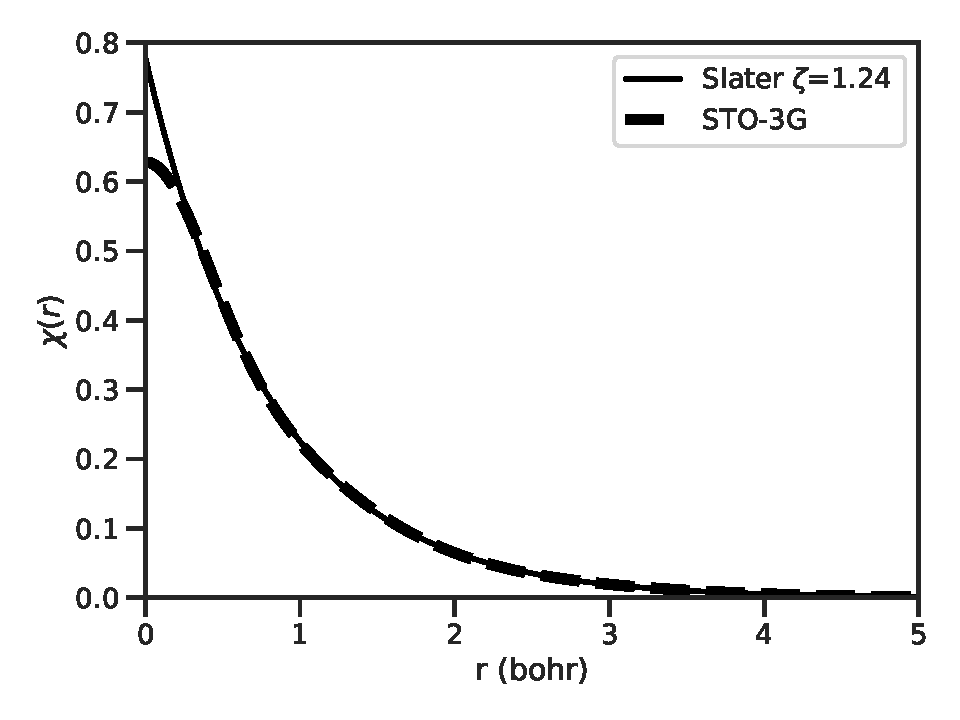
\includegraphics[width=\textwidth]{sto-3g}
\end{minipage}
\caption{STO-3G}
\label{fig:sto-3g}
\end{figure}

For H$_2$, the STO-3G basis consists of only two 1s functions, each centered around a nucleus.
\begin{align}
\left\{\begin{array}{l}
\phi_1(\bs{r}) = \sum\limits_{i=1}^3 c_i \left(\dfrac{2\alpha_i}{\pi}\right)^{3/4} e^{-\alpha_i\vert\bs{r}-\bs{R}_1\vert^2} \\
\phi_2(\bs{r}) = \sum\limits_{i=1}^3 c_i \left(\dfrac{2\alpha_i}{\pi}\right)^{3/4} e^{-\alpha_i\vert\bs{r}-\bs{R}_2\vert^2}
\end{array}\right.,
\end{align}
where $\bs{R}_1=\bs{0}$, and $\bs{R}_2=1.4~\bs{\hat{z}}$ bohr near equilibrium. At 1.4 bohr separation, the kinetic and the electron-ion interaction matrices evaluate to
\begin{align}
T_{\mu\nu}\equiv\braket{\phi_\mu|-\frac{1}{2}\nabla^2|\phi_\nu} =
\left(\begin{array}{cc}
0.76003188 & 0.23645465 \\
0.23645465 & 0.76003188
\end{array}\right), \\
V_{\mu\nu}\equiv\braket{\phi_\mu|\sum\limits_{i=1}^{2}\dfrac{1}{\vert\bs{r}-\bs{R}_i\vert}|\phi_\nu} = \left(\begin{array}{cc}
-1.88044088 & -1.19483461 \\
-1.19483461 & -1.88044088
\end{array}\right),
\end{align}
which sum to the 1-electron hamiltonian $\hcore$ by eq.~(\ref{eq:hf-hcore})

Eigenvectors of $\hcore$ are typically used to construct the initial density matrix to start a self-consist solution of the Hartree-Fock equations. However, in the case of H$_2$, these eigenvectors coincide with the final solution, so we obtain the converged density matrix with no iteration from eq.~(\ref{eq:h2-pmat})
\begin{align}
C_{\mu 1} = \left(\begin{array}{c}
0.70710678 \\ -0.70710678
\end{array}\right);
~P_{\mu\nu} = \left(\begin{array}{cc}
0.60265716 & 0.60265716 \\
0.60265716 & 0.60265716
\end{array}\right).
\end{align}
Finally, we can evaluate the so-called electron repulsion integrals (eris) and the Fock matrix eq.~(\ref{eq:roothaan-fock})
\begin{table}[h]
\centering
\begin{tabular}{ccccc}
\toprule
$\mu$ & $\nu$ & $\lambda$ & $\sigma$ & $(\mu\nu|\lambda\sigma)$\\
\midrule
1 & 1 & 1 & 1 & 0.774605930 \\
1 & 1 & 1 & 2 & 0.444107650 \\
1 & 1 & 2 & 2 & 0.569675915 \\
1 & 2 & 1 & 2 & 0.297028535 \\
\bottomrule
\end{tabular}
\caption{symmetry-inequivalent electron repulsion integrals for H$_2$ in STO-3G.}
\end{table}
\begin{align}
J_{\mu\nu} = \left(\begin{array}{cc}
0.67271523 & 0.44665109 \\
0.44665109 & 0.67271523
\end{array}\right); ~~
K_{\mu\nu} = \left(\begin{array}{cc}
0.59055879 & 0.52880753 \\
0.52880753 & 0.59055879
\end{array}\right);\\
F_{\mu\nu} = \left(\begin{array}{cc}
-0.36553735 & -0.59388537 \\
-0.59388537 & -0.36553735
\end{array}\right).\label{eq:h2-hf-fock-r14}
\end{align}
The total energy is $-1.11671432$ ha, while the electronic contribution is $-1.831$ ha, before adding the ion-ion repulsion $V_{ii}=1/1.4$ ha. Interested reader should reproduce the Fock matrix for STO-3G H$_2$ at 1.4 bohr separation, i.e. eq.~(\ref{eq:h2-hf-fock-r14}), to consolidate a practical understanding of RHF.

\subsubsection{Koopmans Theorem}
Consider removing an electron from orbital $\delta\le N$, the wave function for the $(N-1)$-electron system is~\cite{Giuliani2005}
\begin{align}
\ket{\Psi_{HF}^{(h,\delta)}} = \hat{a}_\delta\ket{\Psi_{HF}}
\end{align}
in the frozen orbital approximation, where the orbitals of the remaining electrons cannot respond to the removed one. The energy of this wave function can be shown to differ from the ground state by $\epsilon_\delta$, the HF eigenvalue of the orbital being emptied.
\begin{align}
E_{HF}^{(h,\delta)} \equiv \braket{\ket{\Psi_{HF}^{(h,\delta)}}|\ham|\ket{\Psi_{HF}^{(h,\delta)}}} = E_{HF} - \epsilon_\delta.
\end{align}
T. Koopmans~\cite{Koopmans1934} first proved this for the highest occupied molecular orbital (HOMO) as an approximation to the ionization energy, although the above derivation is general for any orbital.
Following Chapter 2.2.3 in Ref.~\cite{Giuliani2005}, one can similarly calculate the energy of an N-electron system that differs from the HF ground state by an electron-hole excitation
\begin{align}
\ket{\Psi_{HF}^{(e,\gamma;h,\delta)}} = \hat{a}_\gamma^\dagger \hat{a}_\delta \ket{\Psi_{HF}}, ~\gamma>N,~\delta\le N. \\
E_{HF}^{(e,\gamma;h,\delta)} = E_{HF}+\epsilon_\gamma-\epsilon_\delta-\Delta_{\gamma\delta},
\label{eq:hf-eh}
\end{align}
where $\Delta_{\gamma\delta}>0$. For a stable HF solution, eq.~(\ref{eq:hf-eh}) leads to a \textit{coulomb gap} in the HF density of states in insulators
\begin{align}
N(e) < 2^{d-1}d\left(\dfrac{\epsilon}{e^2}\right)^d(e-e_F)^{d-1},
\end{align}
where $d$ is the number of spatial dimensions, and $\epsilon$ is the dielectric constant of the insulator. That is, the HF density of states must vanish at least as fast as $(e-e_F)^{d-1}$ around the Fermi energy $e_F$.

Koopmans theorem assigns physical meanings to the HF eigenvalues, but is only applicable relative to the HF ground state. For example, one cannot repeatedly apply Koopmans theorem to reconstruct the total energy of the system by stripping one electron at a time. The sum of HF eigenvalues double counts the interaction energy, which must be subtracted to calculate the HF total energy
\begin{align}
E_{HF} = \sum\limits_{\alpha} n_\alpha \epsilon_\alpha - \frac{1}{2}n_\alpha (V_{\alpha\alpha}^{HF}-V_{\alpha\alpha}^{ext}).
\end{align}

\subsubsection{Basis Set Error}

\subsubsection{Beyond Hartree-Fock}
Even when the complete basis set limit is reached, the HF solution is still not the exact electronic ground state due to its neglect of electron correlation.
The virtual orbitals can be used to construct N-electron determinants that differ from the HF ground state by changing orbital occupation.
These determinants form a many-body basis, in which any wave function can be expressed as a linear combination.
This leads to the configuration interaction (CI) expansion, where the exact electronic ground state is expanded in many-body bases of increasing sizes
\begin{align} \label{eq:method-hf-ci}
\psi_0 = \lim\limits_{M\rightarrow\infty}\sum\limits_{i=0}^{M} c_i \ket{D_i}.
\end{align}
If all determinants that differs by one particle-hole excitation from reference are considered, then we obtain a CI singles (CIS) expansion. If these, and all determinants with two particle-hole excitations are considered, then the expansion is CI singles and doubles (CISD), etc..

\subsubsection{Static and Dynamic Correlation}
The ground state is said to have \textit{static correlation} if one or more determinants in the exact expansion eq.~(\ref{eq:method-hf-ci}) are nearly degenerate with the reference determinant.
This will happen if there are virtual orbitals nearly degenerate with the highest occupied molecular orbital.
In contrast, the system has \textit{dynamic correlation} if the $c_i$ coefficients are small but non-zero for many determinants with high levels of excitation.
Dynamic correlation is often attributed to strong local correlation such as the electron-electron cusp condition.
The exact definitions of static and dynamic correlations are still murky~\cite{Benavides-Riveros2017}.
I introduce the above working definitions, because the static correlation can be interpreted as a delocalization error due to fractional electron~\cite{Cohen2008}, and is related to the self-interaction error in density functional theory (DFT).
This bridges the languages used in quantum chemistry and condensed matter and points to a solution of the infamous ``bandgap problem'' to be introduced in  Sec.~\ref{sec:method-dft-bandgap}.

\subsection{Kohn-Sham Density Functional Theory (KS-DFT)}
While the Hartree-Fock method enjoys much success in the study of atoms and molecules, its complete neglect of (Coulomb) electron correlation is woefully inadequate for many solids. The total energy is dominated by inner shell contributions, which overshadow the valence contributions important for bonding and correlated excitations in solids. The HF energy eigenvalues show vanishing density of states at the Fermi level in metals and unphysically large band gaps in insulators~\cite{Perdew1981}.

Density functional theory uses the three-dimensional total electron density $n(\bs{r})$ as the basic variable rather than the 3N-dimensional many-body wave function $\Psi(\bs{r}_1,\dots,\bs{r}_N)$. This is a dramatic simplification that likely lead to its dominance in modern electronic structure theory of solids and material science.

\subsubsection{The Hohenberg-Kohn theorems}
While having roots in Thomas-Fermi theory~\cite{Parr1989}, DFT was put on firm theoretical foundation by P. Hohenberg and W. Kohn (HK) in 1964~\cite{Hohenberg1964}, where they calculate the total energy $E$ from an external potential $v(\bs{r})$ and a functional of the ground-state electron density
\begin{align}
E\equiv \int d\bs{r} n(\bs{r}) v(\bs{r}) + F[n(\bs{r})].
\end{align}
Two theorems are often attributed to this work:
\begin{definition}
\textit{V-representable density} A density $n(\bs{r})$ is V-representable if it is the ground-state density of some Hamiltonian $H$ in an external potential $v(\bs{r})$.
\end{definition}
\begin{theorem}
Assuming non-degenerate ground state, any V-representable ground-state density $n(\bs{r})$ uniquely determines its external potential $v(\bs{r})$. %(See extension to N-representable density by M. Levy)
\end{theorem}
\begin{proof}
by contradiction: Suppose there are two distinct external potentials $v$ and $v'$ that give rise to the same density $n$ via different hamiltonians $H$, $H'$ and wave functions $\Psi$ and $\Psi'$, respectively. By the variational principle $\braket{\Psi'|H'|\Psi'}+\braket{\Psi'|v'-v|\Psi'}=\boxed{\braket{\Psi'|H|\Psi'}>\braket{\Psi|H|\Psi}}=\braket{\Psi|H'|\Psi}+\braket{\Psi|v'-v|\Psi}>\braket{\Psi'|H'|\Psi'}+\braket{\Psi|v'-v|\Psi}$. Since $\Psi$ and $\Psi'$ give the same density, the local term $\braket{v'-v}$ cancels to give $\braket{\Psi'|H'|\Psi'}>\braket{\Psi'|H'|\Psi'}$, which is a contradiction.
\end{proof}
\begin{theorem}
Assuming number-conserving density variations that retain V-representability, the energy functional has a unique minimum at the ground-state density.
\end{theorem}
\begin{proof}
Consider an external potential $v$, its hamiltonian $H$, and its unique ground state $\Psi$ and density $n$. After a number-conserving variation, the new wave function $\Psi'$ can be used with the original hamiltonian and $\braket{\Psi'|H|\Psi'}>\braket{\Psi|H|\Psi}$ by the variational principle.
\end{proof}

These initial proofs by HK have two important assumptions: 1. the ground-state is non-degenerate and 2. the electron density $n(\bs{r})$ is V-representable. The latter is especially sever because reasonable densities were shown to be not V-representable~\cite{Levy1982,Lieb1983}. Fortunately, M. Levy proved that both assumptions can be weakened~\cite{Levy1979}.
\begin{definition}
\textit{N representable density} A density $n(\bs{r})$ is N-representable if it can be obtained from some anti-symmetric wave function.
\end{definition}
The HK theorems hold for N-representable densities regardless of ground-state degeneracy.

While less publicized, HK also pointed out that the exact density functional less the direct/Column contribution can be calculated from a local energy-density functional $g_{\bs{r}}[n]$
\begin{align}
G[n]\equiv F[n]-\frac{1}{2}\int d\bs{r}d\bs{r}' \dfrac{n(\bs{r})n(\bs{r}')}{\vert\bs{r}-\bs{r}'\vert}=\int \bs{r} g_{\bs{r}}[n],\\
g_{\bs{r}}[n] \equiv \frac{1}{2}\nabla_{\bs{r}}\nabla_{\bs{r}'} n_1(\bs{r}, \bs{r}')\vert_{\bs{r}=\bs{r}'}+
\frac{1}{2}\int d\bs{r}' \dfrac{C_2(\bs{r}-\bs{r'}/2;\bs{r}+\bs{r}'/2)}{\vert\bs{r}'\vert},
\end{align}
which is constructed from one- and two-body reduced density matrices $n_1$ and $C_2$. They even went as far as to relate the leading-order behavior of the density functional to polarizability
\begin{align}
G[n] = G[n_0] + \int d\bs{r}d\bs{r}' K(\bs{r}-\bs{r}')\tilde{n}(\bs{r})\tilde{n}(\bs{r}')+h.o.,
\end{align}
where $\tilde{n}$ is a small number-conserving density variation and the kernel $K$ is related to the polarizability in reciprocal space
\begin{align}
K(\bs{r}-\bs{r}') = \dfrac{1}{\Omega}\sum\limits_{\bs{q}} K(\bs{q}) e^{-i\bs{q}\cdot(\bs{r}-\bs{r}')}, \\
K(\bs{q}) = \dfrac{2\pi}{q^2}\left[ \frac{1}{\alpha(\bs{q})}-1 \right] = \dfrac{2\pi}{q^2}\dfrac{1}{\epsilon(\bs{q})},
\end{align}
where $\alpha(\bs{q})$ and $\epsilon(\bs{q})$ are the polarizability and dielectric constant, respectively. The HK theorems and limits provide some checks for practical parametrization of the exact density functional. Unfortunately, they provide no guidance on how one might start to construct numerical approximations to the exact functional.

\subsubsection{The Kohn-Sham equations}

One year after the HK paper, W. Kohn and L. J. Sham (KS)~\cite{Kohn1965} worked out practical guidelines for constructing approximations to the exact density functional. KS first partitioned the total energy to highlight the least-understood ``exchange-correlation" term $E_{xc}[n]$.
\begin{align} \label{eq:ks-etot}
E=\int d\bs{r} n(\bs{r}) v(\bs{r}) + \frac{1}{2}\int d\bs{r}d\bs{r}' \dfrac{n(\bs{r})n(\bs{r}')}{\vert\bs{r}-\bs{r}'\vert} + T[n] + E_{\text{xc}}[n],
\end{align}
where $T$ is a kinetic energy functional. KS then approximated $E_{xc}$ by the corresponding contribution in the homogeneous electron gas, the local density approximation (LDA)
\begin{align}
E_{\text{xc}}[n] = \int d\bs{r}n(\bs{r})\epsilon_{\text{xc}}(n(\bs{r})).
\end{align}
Next, by minimizing eq.~(\ref{eq:ks-etot}) with respect to number-conserving density variation, they obtained the stationary condition for the ground-state density
\begin{align}
\int \delta n \left[
\dfrac{\delta T[n]}{\delta n}+
v(\bs{r}) + \int d\bs{r}' \dfrac{n(\bs{r}')}{\vert\bs{r}-\bs{r}'\vert}+
\dfrac{d(n\epsilon_{\text{xc}}(n))}{dn}
\right] = 0. \label{eq:ks-dn}
\end{align}
To solve eq.~(\ref{eq:ks-dn}), KS \textit{assumed} that the ground-state density $n$ came from an auxiliary system of non-interacting electrons, i.e., a Slater determinant. This KS \textit{ansatz} turns eq.~(\ref{eq:ks-dn}) into a system of one-particle equations of non-interacting particles in some effective potential $v^{\text{eff}}_{KS}$ determined by the density $n(\bs{r})$. Most practical implementations of DFT use the KS auxiliary-system formulation.

Practical success of the DFT LDA method was not realized until 1981, when J. P. Perdew and A. Zunger~\cite{Perdew1981} (PZ) parametrized exact quantum Monte Carlo data of the homogeneous electron gas, obtained by D. M. Ceperley and B. J. Alder~\cite{Ceperley1980} the year prior. PZ's eq.~(13-17) define the KS-DFT method and the LDA we use today. The electron density for spin $\sigma$ is a sum of occupied spin orbitals squared
\begin{align}
n_{\sigma} = \sum\limits_{\sigma}\sum\limits_{a=1}^{N_{\sigma}}
f_{a\sigma} \vert\psi_{a\sigma}(\bs{r})\vert^2,
\end{align}
where the occupation numbers $f_{a\sigma}\in[0, 1]$, and the kinetic energy is the sum of contributions from all occupied spin orbitals
\begin{align}
T[n] = \sum\limits_\sigma\sum\limits_{a=1}^{N_{\sigma}}
f_{a\sigma} \braket{\psi_{a\sigma}|-\frac{1}{2}\nabla^2|\psi_{a\sigma}}.
\end{align}
Minimizing eq.~(\ref{eq:ks-etot}) with the constraint that the spin orbitals remain orthonormal, PZ obtains
\begin{align}
\dfrac{\delta}{\delta\psi_{a\sigma}} \left[
T[n] + \int d\bs{r}v(\bs{r}) + \int d\bs{r}\int d\bs{r}' \dfrac{n(\bs{r}')}{\vert\bs{r}-\bs{r}'\vert} +
\dfrac{\delta}{\delta n_{\sigma}} E_{xc}(n_{\up},n_{\dn})
\right]
\end{align}

\subsubsection{Minimum Basis H$_2$}
In the PZ formulation of KS-DFT, the only difference between the LDA and the RHF calculations lies in the ``exchange'' matrix
\begin{align}
K_{\mu\nu}' = \left(\begin{array}{cc}
0.38980073 & 0.25499926 \\
0.25499926 & 0.38980073
\end{array}\right)\\
F_{\mu\nu} = \left(\begin{array}{cc}
-0.16477935 & -0.32007715 \\
-0.32007715 & -0.16477935
\end{array}\right).\label{eq:h2-lda-fock-r14}
\end{align}
The LDA electronic contribution is $-1.73929592$ ha.

\subsubsection{The Band Gap Problem} \label{sec:method-dft-bandgap}
The Kohn-Sham eigenvalues do not have the same physical meaning as the Hartree-Fock eigenvalues as given by Koopmans theorem. Thus, a band gap ``problem'' arises when one compares the HOMO-LUMO gap from KS-DFT to experimental measurements of the fundamental gap $E_g$. When extended to handle systems with fractional electron number, the derivative discontinuity of the exact density functional is equal $E_g$. It has contribution from both the non-interacting kinetic functional $T_s[n]$ and the exact exchange-correlation functional $E_{xc}[n]$. The KS HOMO-LUMO gap measures the derivative discontinuity in $T_s[n]$. However, as shown in Fig.~\ref{fig:method-dft-smooth-lda}, in the LDA, $E_{xc}[n]$ is smooth, so its contribution to the gap is missing. As a result, the LDA gap is $\sim 50\%$ that of experiment, showing that the derivative discontinuity in $E_{xc}[n]$ can be of similar magnitude as the gap and cannot be ignored.

\begin{figure}[h]
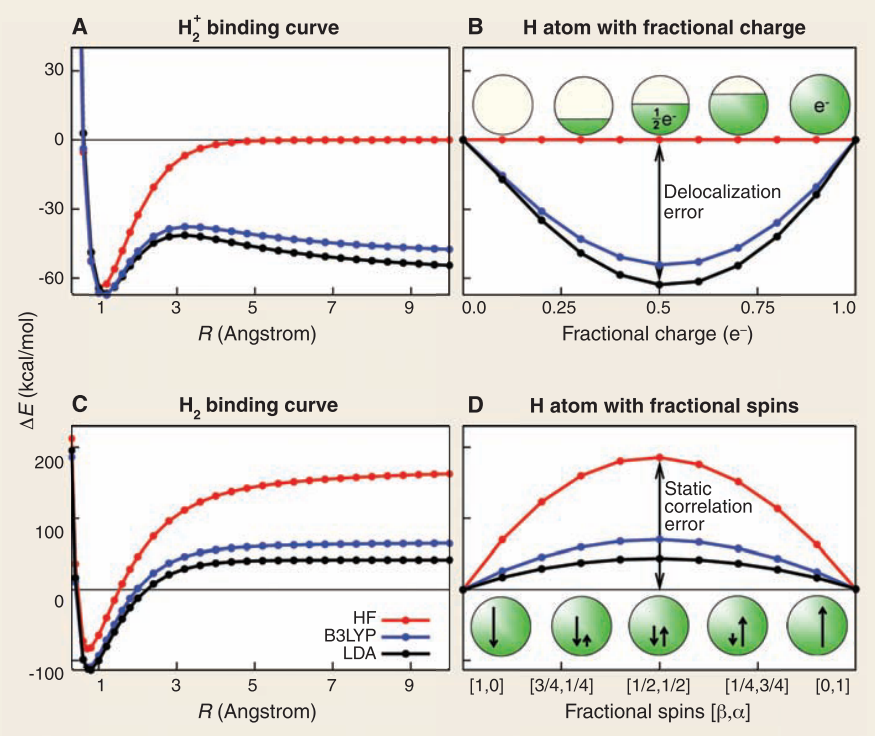
\includegraphics[width=0.45\linewidth]{cohen2008-fig1}
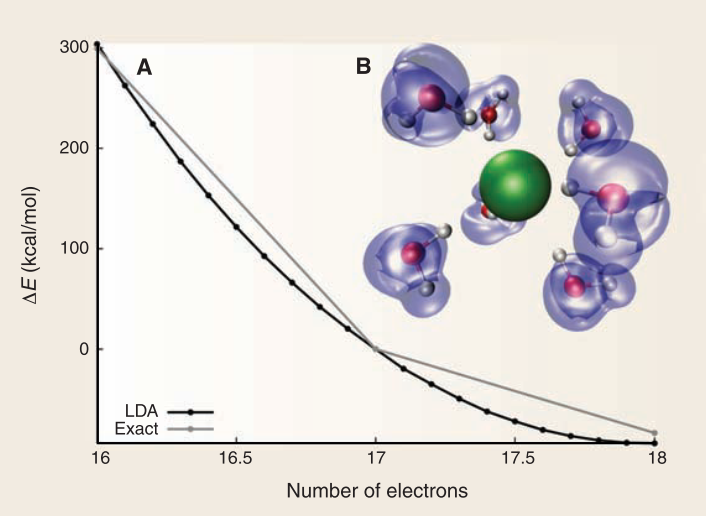
\includegraphics[width=0.52\linewidth]{cohen2008-fig2}
\caption{A. J. Cohen, P. Mori-S\'anchez, and W. Yang~\cite{Cohen2008} explains the self-interaction error in H$_2$ binding curve (left panel C and D) due to the presence of fractional electron (left panel B), which leads to a delocalization error when LDA is used (right panel).}
\label{fig:method-dft-smooth-lda}
\end{figure}

% Q/ why is HSE so good?
% A/ because it has both convex and concave components. See Cohen 2008 Fig. 2

\subsubsection{Beyond Local Density Approximation}

generalized gradient approximation (PBE and BLYP)

van der Waals functionals (vdW-DF)

exact exchange functionals (HSE)

SCAN?